\documentclass[border=10pt]{standalone}
\usepackage[svgnames]{xcolor}
\usepackage{amsmath}
\usepackage{pgfplots}
\pgfplotsset{compat=newest}
\usepackage[sfdefault]{FiraSans}
\usepackage{FiraMono}
\renewcommand*\familydefault{\sfdefault}
\begin{document}
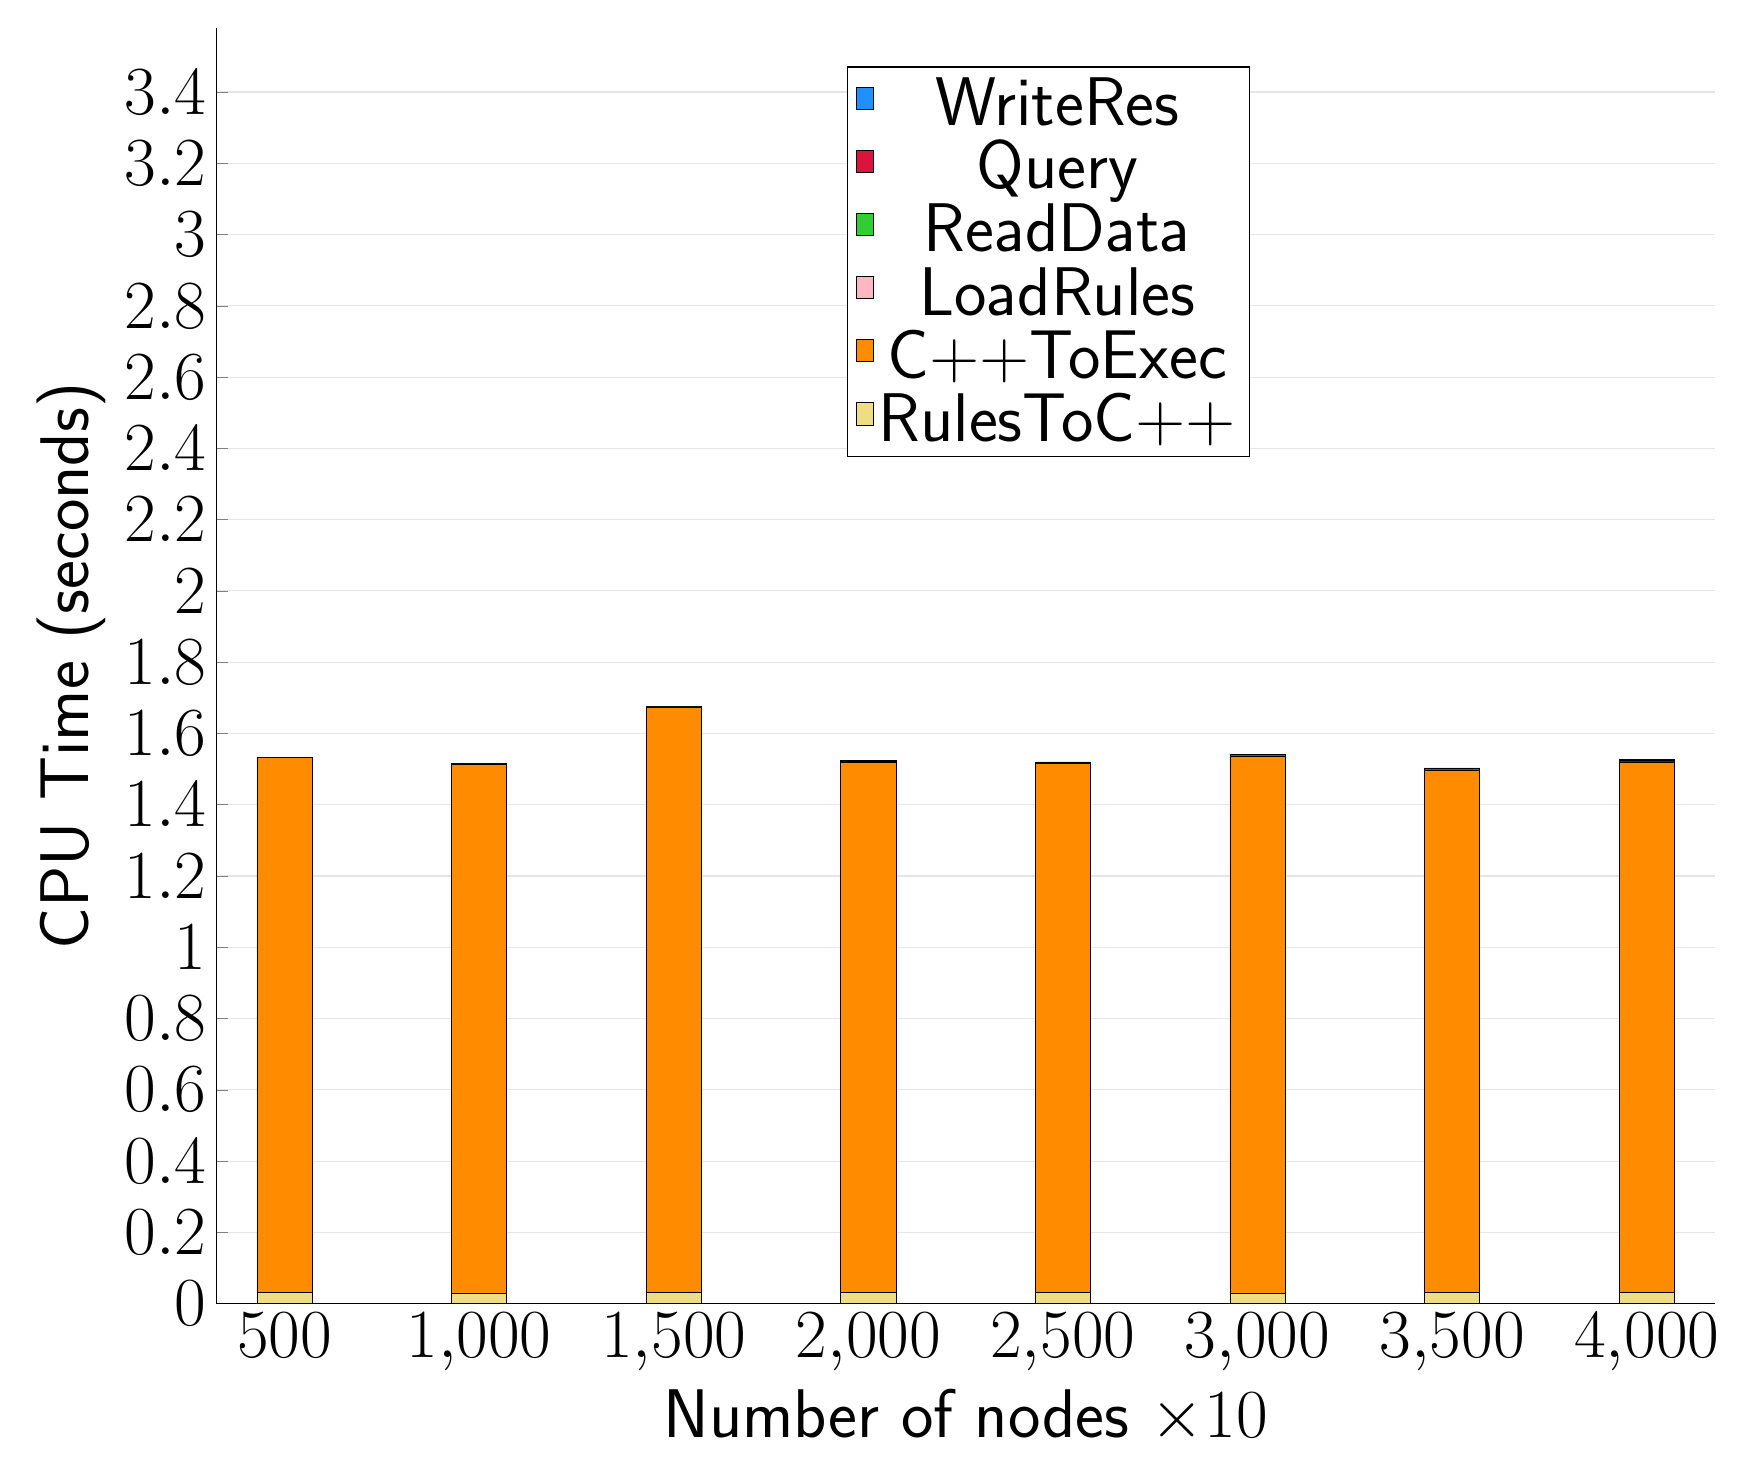
\begin{tikzpicture}
\begin{axis}[
   ybar stacked,
   width=1.7\textwidth,
   bar width=0.7cm,
   ymajorgrids, tick align=inside,
   major grid style={draw=gray!20},
   xtick=data,
   ymin=0, ymax=3.579,
   axis x line*=bottom,
   axis y line*=left,
   enlarge x limits=0.05,
   legend style={
       at={(0.69, 0.97)},
       anchor=north east,
       legend columns=1,
       font=\Huge,
   },
   ylabel={CPU Time (seconds)},
   xlabel={Number of nodes $\times 10$},
   label style={font=\Huge},
   tick label style={font=\Huge},
]
\addlegendimage{fill=DodgerBlue, draw=black, line width=0.2pt}
\addlegendentry{WriteRes}
\addlegendimage{fill=Crimson, draw=black, line width=0.2pt}
\addlegendentry{Query}
\addlegendimage{fill=LimeGreen, draw=black, line width=0.2pt}
\addlegendentry{ReadData}
\addlegendimage{fill=LightPink, draw=black, line width=0.2pt}
\addlegendentry{LoadRules}
\addlegendimage{fill=DarkOrange, draw=black, line width=0.2pt}
\addlegendentry{C++ToExec}
\addlegendimage{fill=LightGoldenrod, draw=black, line width=0.2pt}
\addlegendentry{RulesToC++}
\addplot +[fill=LightGoldenrod, draw=black, line width=0.2pt] coordinates {
(500, 0.031000000000000007)
(1000, 0.030000000000000006)
(1500, 0.031000000000000007)
(2000, 0.031000000000000007)
(2500, 0.031000000000000007)
(3000, 0.030000000000000006)
(3500, 0.031000000000000007)
(4000, 0.031999999999999994)
};
\addplot +[fill=DarkOrange, draw=black, line width=0.2pt] coordinates {
(500, 1.501)
(1000, 1.483)
(1500, 1.6430000000000002)
(2000, 1.4880000000000002)
(2500, 1.4840000000000002)
(3000, 1.5059999999999998)
(3500, 1.465)
(4000, 1.4880000000000002)
};
\addplot +[fill=LightPink, draw=black, line width=0.2pt] coordinates {
(500, 0.00010320000000000001)
(1000, 0.00010799999999999998)
(1500, 0.0)
(2000, 0.00012440000000000004)
(2500, 9.87e-05)
(3000, 0.0001093)
(3500, 0.0001248)
(4000, 6.15e-05)
};
\addplot +[fill=LimeGreen, draw=black, line width=0.2pt] coordinates {
(500, 0.00034520000000000004)
(1000, 0.0004666999999999999)
(1500, 0.00039789999999999997)
(2000, 0.0007125)
(2500, 0.0007843000000000001)
(3000, 0.0008927000000000001)
(3500, 0.0010725)
(4000, 0.0010450999999999998)
};
\addplot +[fill=Crimson, draw=black, line width=0.2pt] coordinates {
(500, 0.0006115)
(1000, 0.0012253)
(1500, 0.0011457)
(2000, 0.002521)
(2500, 0.0029353)
(3000, 0.0035470999999999996)
(3500, 0.0044519)
(4000, 0.0045708)
};
\addplot +[fill=DodgerBlue, draw=black, line width=0.2pt] coordinates {
(500, 0.0004273000000000001)
(1000, 0.0006885)
(1500, 0.000662)
(2000, 0.0012106000000000003)
(2500, 0.0012556)
(3000, 0.001518)
(3500, 0.0018306000000000004)
(4000, 0.0018499999999999999)
};
\end{axis}
\end{tikzpicture}

\end{document}
